\chapter{Project}

This section will discuss the entities and requirements evaluated from the proposal.
\todo{e o design geral do project, overview das seccoes}

\section{Requirements}
Given the written proposal and eventual consultations with stakeholders, the general behavior and requirements of this application were evaluated. In regards to use cases, two actors were identified, a User that represents professors and employees that belongs to \gls{IPB} and a Administrator that manages the state of the application.

As an authenticated User, there are two goals that are covered by the use-case diagram shown in Figure~\ref{fig:userusecase}, to ``Run'' a Query and to Export a Spreadsheet. The former refers to when a User only wants to have some of the institution's information for a brief period of time and the latter, even though taking the same steps, provides the user with a spreadsheet file to be downloaded.

An authenticated Administrator, because he is expected to manage the system, is provided of more use-cases that follow a similar pattern, that is, managing the entities that compose the system by the means of \gls{CRUD} operations. Added to this, the use-case diagram found in Figure~\ref{fig:adminusecases} raises action ``Associate User and Permission'' that indicates the process of enabling an User to run a Query.

Alongside the use cases just evaluated, the project proposal expresses the following requirements:
\begin{enumerate}
\item The system should be able to run queries in the database currently employed at the institution.\label{req:multidb}
\item Users can only run queries in which they have Permission to.\label{req:permission}
\item Query commands may be longer than 30 lines long.\label{req:longquery}
\item Running a Query yields a table that can be downloaded.\label{req:download}
\item No \gls{SQL} knowledge is needed to execute a Query.\label{req:noknowledge}
\item The system enables the insertion of new Queries.\label{req:addquery}
\end{enumerate}

\begin{figure}
  \centering
  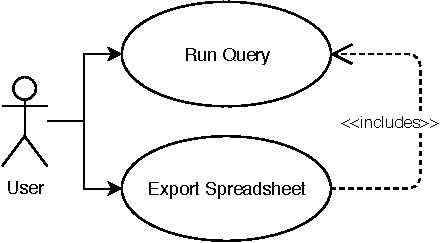
\includegraphics[width=.5\textwidth]{images/diagramas/userusecase}
  \caption{User use-case}\label{fig:userusecase}
\end{figure}

\begin{figure}
  \centering
  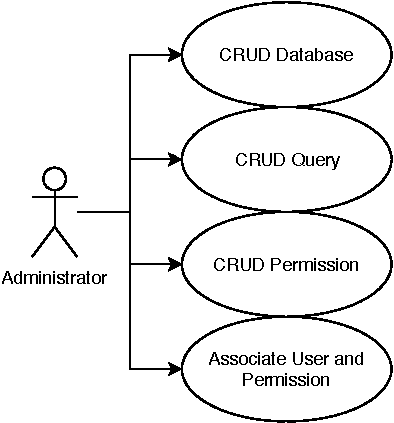
\includegraphics[width=.5\textwidth]{images/diagramas/adminusecase}
  \caption{Administrator use-cases}\label{fig:adminusecases}
\end{figure}

Based on the artifacts evaluated so far, four entities were found to model the data that surrounds the application. Because these entities function more as information aggregates and do not exchange messages, they are better expressed through a Entity Relational diagram as seen in Figure~\ref{fig:er}. What follows is a description of each evaluated entity and their functional relation.

\begin{description}
\item[Database] Where a Query is run.\\
  It is responsible to hold the information that enables the access to a given database, effectively meeting requirement~\ref{req:multidb}.
  In the most basic form, a connection requires the network address and authentication credentials.
\item[Query] A script that is run in a Database and gather information into a single table.\\
  A \gls{SQL} script must be issued during a session with a Database.
  To fulfill requirement~\ref{req:noknowledge}, some meta information such as a title and a description so that the target audience is able to find the Query that fulfill their needs.
\item[Permission] The binding between Users and Queries.\\
  In order to fulfill requirement~\ref{req:permission}, this entity is responsible to handle the relation between a User and all the Queries that they may access.
\item[User] Represents the person currently logged-in.\\
  It has two purposes, first is to differentiate users according to their roles, either ``Administrators'' or ``User'' so that certain actions are disabled, for example the Administrative task stated in requirement~\ref{req:addquery}
  The second is to be used when filtering Queries so that requirement~\ref{req:permission}
\end{description}

This application's architecture was heavily influenced by the non-functional requirement of being easily maintained by the institution's \gls{IT} department given that most of their currently developed systems are composed of a two part application composed of a Web front-end that fetches information from a back-end \gls{API}, referred in Figure~\ref{fig:overview} as ``\gls{Yabi} Front-end'' and ``Yabi Back-end'', respectively.
Also note that what is considered as \gls{Yabi} or ``the application'' encompass both front and back ends and a \gls{RDBMS}.

Figure~\ref{fig:overview} also provide in broad terms the elements that the application interacts directly with. The back-end being responsible for authenticating users on the Directory Service, managing and persisting entities on a \gls{RDBMS} and running Queries on remote databases. Actors interact solely through \gls{Yabi} front-end.

\begin{figure}
  \centering
  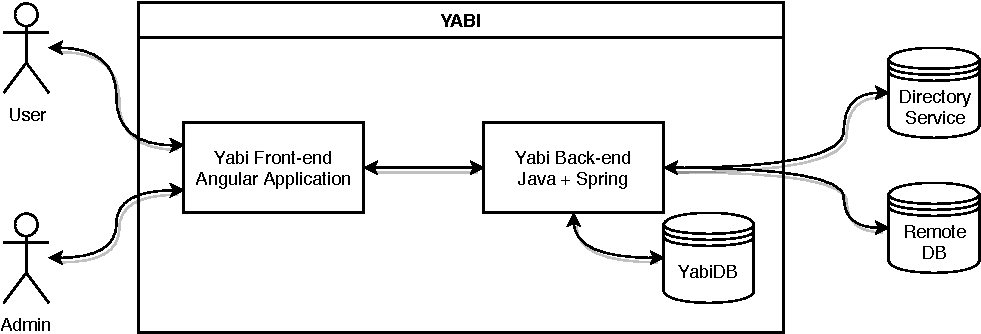
\includegraphics[width=\textwidth]{images/diagramas/overview.pdf}
  \caption{Yabi Overview}\label{fig:overview}
\end{figure}

\section{Project Details}
Due to the how the entities and their relations were designed, it is important to note some peculiarities and restrictions that came with it.

To begin with, Queries must be associated to only one Permission, avoiding repetitions when listing an User's available Queries.

Users have a many to many relation to Permission, therefore they may have more than one permission and have access to a custom set of Queries.

An Administrator can manage all parts that are within the application's domain, because of this they cannot change the username as it is bound to the Directory Service.

Permissions is a central piece of this system and it's what associates users with information.
They follow a hierarchy structure with a root Permission whose path is simply ``/'' and its parent is itself.
A child Permission has its \texttt{nodepath} beginning with the content of their parent's \texttt{nodePath}.

There are only two roles that any given user may be assigned to, either Administrator or User.

\section{Entity Relations Diagram}\label{tities}
When implementing the entities that were previously evaluated, it was found that some of the proposed names were reserved to \gls{RDBMS} and synonyms had to be used in the back-end, therefore Query became \texttt{SqlQuery} and Database became \texttt{Directory}. Permission is a separate case as its implementation name was supposed to represent their tree-like nature and was thus it was named \texttt{PermissionTree}.

Figure~\ref{fig:er} show the relations between the implemented entities. The shape of the arrows indicate the cardinality of the relation.

\begin{figure}
  \centering
  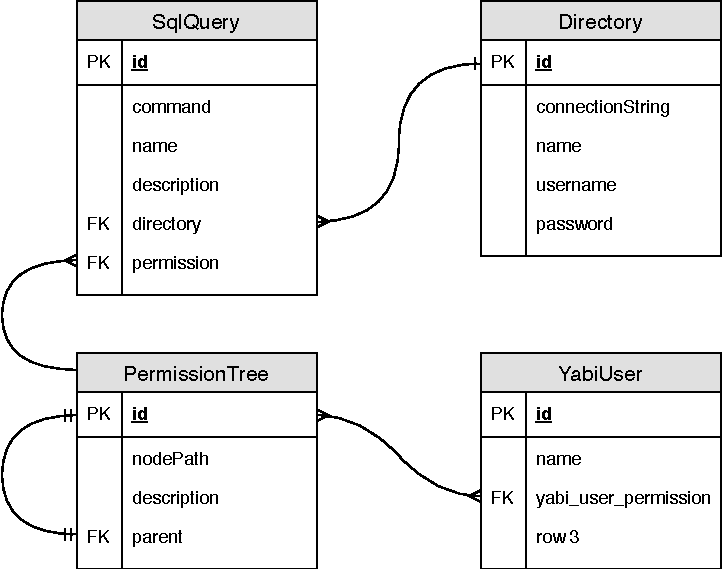
\includegraphics[width=.7\textwidth]{images/diagramas/er}
  \caption{Entity Relational Diagram}\label{fig:er}
\end{figure}

\subsection{Query}\label{model:query}
Implemented in the back-end as \texttt{SqlQuery}, this entity has a Many-to-One relation with \texttt{Directory}. In other words, many Queries may run on the same Database. The relation to \texttt{PermissionTree} is of similar constraints so that many entries of Query may reference the same permission.

\subsection{Database}
Database was implemented as \texttt{Directory} because of a name clash with the \gls{RDBMS}'s repository reserved words. They have no reference of their own, being one of the most simple entities in relation to the others.

\subsection{Permission}

Permission plays a vital role in this architecture. As shown in Figure~\ref{fig:er}, it is the connecting element between Queries and Users. This is the basis for the Permission-based authorization.

One interesting aspect is that every \texttt{PermissionTree} must have a reference to its parent, no exception. This leads to a cyclic reference on the root node. Deleting a permission implies the cascade to all of its children.
\todo{O no raiz deve sempre existir, as permissoes sao pendiradas na arvore e a raiz precise ser boostrapped no deploy. se a raiz for deletada, nao tem como adicionar mais permissoes.}
\subsection{User}\label{model:user}

\section{Authentication and Authorization}\label{proj:auth}
As seen o Figure~\ref{fig:overview}, the authentication is made in the remote Directory Service. 

\section{Template Sb-Admin-Material}
The design of the Web \gls{UI} was not planned to change. 